\subsection{系統概述}

本系統包含兩個主要的使用情境:「使用者個人資訊與情報的建立與管理」以及「成員之間的互動論壇」。兩者之使用情境如圖~\ref{pic:use:userLogin} 與圖~\ref{pic:use:forum}。

\begin{figure}[H]
\centering
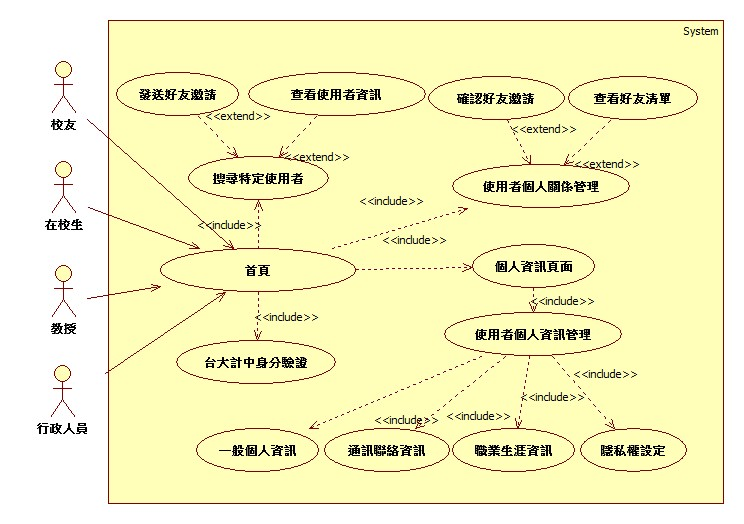
\includegraphics[width=.95\textwidth]{img/useseq/stage1/userProfile.jpg}
\caption{Use Case Diagram -- 使用者資訊管理}
\label{pic:use:userLogin}
\end{figure}

\begin{figure}[H]
\centering
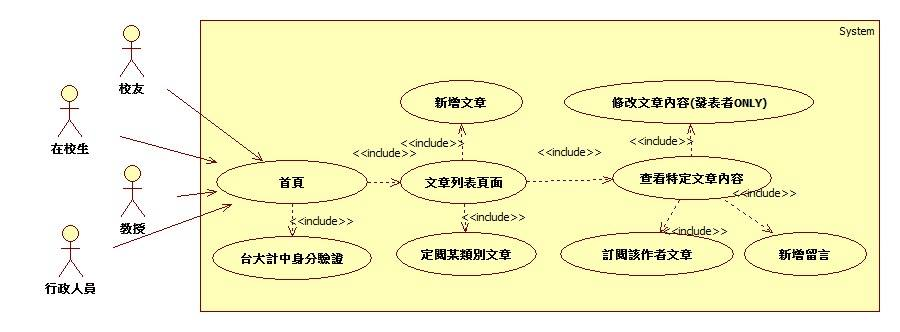
\includegraphics[width=1.05\textwidth]{img/useseq/stage2/useForum.jpg}
\caption{Use Case Diagram -- 文章與留言管理}
\label{pic:use:forum}
\end{figure}

以下之各小節將會逐一介紹各模組之功能及其設計概念。

%% ####################### %%
\subsubsection{登入模組}
在登入模組中需包含以下幾點功能: 
\begin{itemize}
\item{宣稱身分}
\item{身分認證}
\item{取得回傳之 token 並解構}
\end{itemize}
在宣稱身分的地方必須由使用者宣稱自己的身分並提供相關認證資料,在經由計算機中心所提供之 single sign-on 之服務完成身分認證之後,回傳給系統一組經認證的特定格式之 Token。若使用者為初次登入本系統,則此 Token 在經系統解構之後必須能夠抽取部分必要資料填入系統之資料庫中做為使用者個基礎資訊。此行為將於前端網頁系統中完成,若有需要填入時則會交由後端資料系統負責。使用者與系統之間的互動請參考圖~\ref{pic:seq:login}。

\begin{figure}[H]
\centering
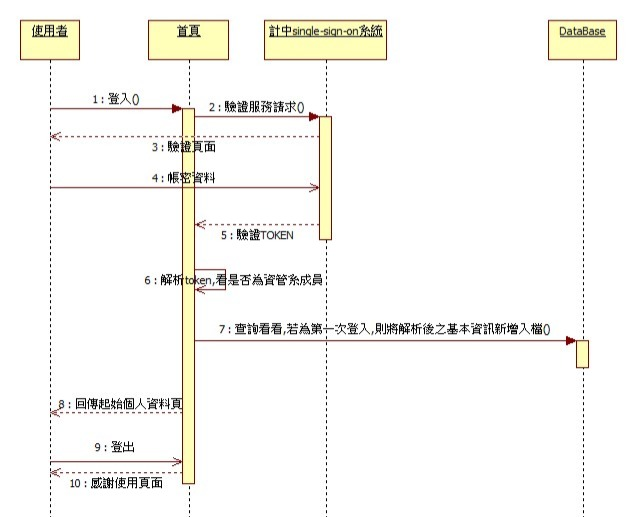
\includegraphics[width=.85\textwidth]{img/useseq/stage1/seqLogin.jpg}
\caption{Sequence Diagram -- 首頁登入}
\label{pic:seq:login}
\end{figure}

%% ####################### %%
\subsubsection{個人資料管理模組}

\begin{figure}[H]
\centering
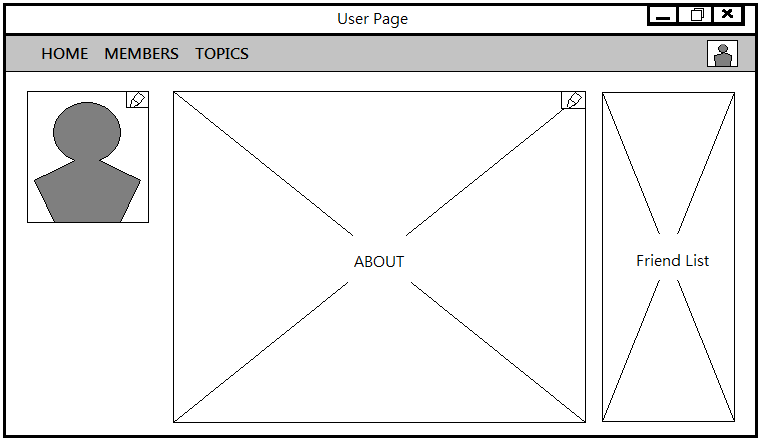
\includegraphics[width=0.7\textwidth]{img/prototype/UserPage.png}
\caption{Prototype -- 用戶資訊頁面}
\label{pic:pro:profile}
\end{figure}

個人資料管理模組將負責管理每個使用者各自的資料組,此資料組中包含使用者的公開資料、個人連絡資料、職業生涯相關資料與隱私權管理及關係管理。使用者必須能夠看見目前系統內的資料狀況並且能夠更動大部分的資料,其中如學號等等的則必須要經過系統管理者之認證後方可變更。此更改之行為將於前端網頁系統中完成,若有資料必須儲存則會交由後段資料系統負責。使用者與系統之間的互動請參考圖~\ref{pic:seq:profileMgt}。此功能會產生一系列之獨立頁面以便於瀏覽與修改個人資訊,雛形如圖~\ref{pic:pro:profile} 所示。

\begin{figure}[H]
\centering
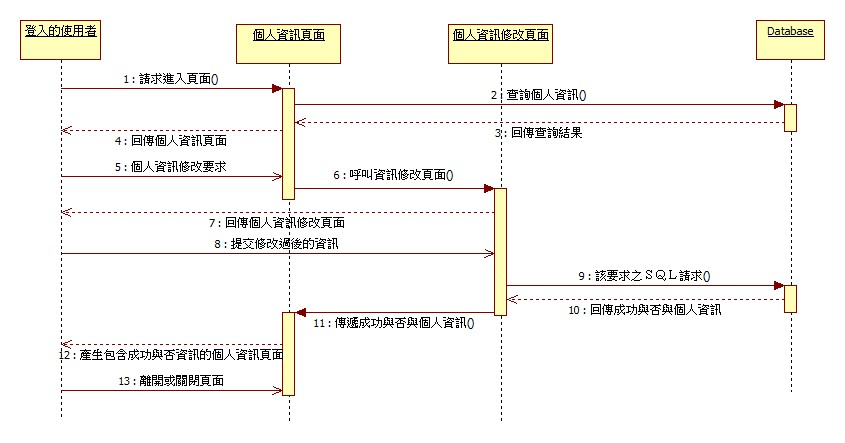
\includegraphics[width=\textwidth]{img/useseq/stage1/seqProfileEdit.jpg}
\caption{Sequence Diagram -- 個人資訊管理與個人資訊修改}
\label{pic:seq:profileMgt}
\end{figure}

%% ####################### %%
\subsubsection{搜尋模組}
本系統為了建立一個適合使用者相互溝通之平台,必須提供使用者方便互相連結之功能,搜尋模組正是為了此需求所建立。當使用者在討論區中產生對特定用戶之好奇心,便可藉由本模組使用特定資料(如:學號)做為索引找到該用戶之公開資訊。公開程度將依該用戶之隱私設定做限制,若該用戶認為預設之帳號類別方式無法達成所欲之特殊公開之組合則需透過朋友關係的建立來達成要求。互相成為朋友的兩人將以特別規則優於普通規則的方式優先採用該用戶所設定的特別規則觀看公開資訊。本搜尋功能將全部於前端網頁系統完成。使用者與系統之間的互動模式請參考圖~\ref{pic:seq:searchUser} ,可產出之相對網頁原形 (prototype) 如圖~\ref{pic:pro:memberList} 。

除了使用者搜尋之外,如圖~\ref{pic:use:forum} 中的「文章列表頁面」以及「查看特定文章內容」等部分所描述之情境,系統也允許使用者針對文章或是文章分類去進行搜尋。與此功能相對之網頁原形 (prototype) 如圖~\ref{pic:pro:articleList} 。

\begin{figure}[H]
\centering
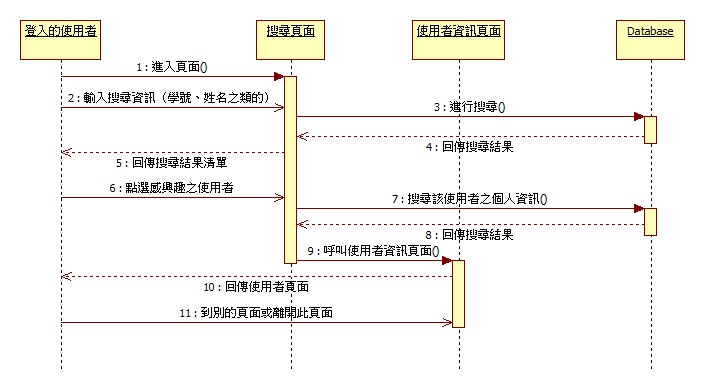
\includegraphics[width=\textwidth]{img/useseq/stage1/seqSeqrchUser.jpg}
\caption{Sequence Diagram -- 搜尋查看他人使用者資訊}
\label{pic:seq:searchUser}
\end{figure}

\begin{figure}[H]
\centering
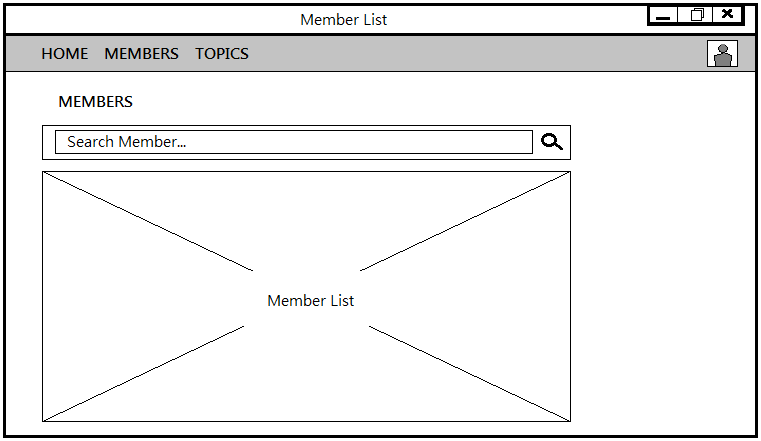
\includegraphics[width=.7\textwidth]{img/prototype/MemberList.png}
\caption{Prototype -- 使用者列表頁面(含搜尋功能)}
\label{pic:pro:memberList}
\end{figure}

\begin{figure}[H]
\centering
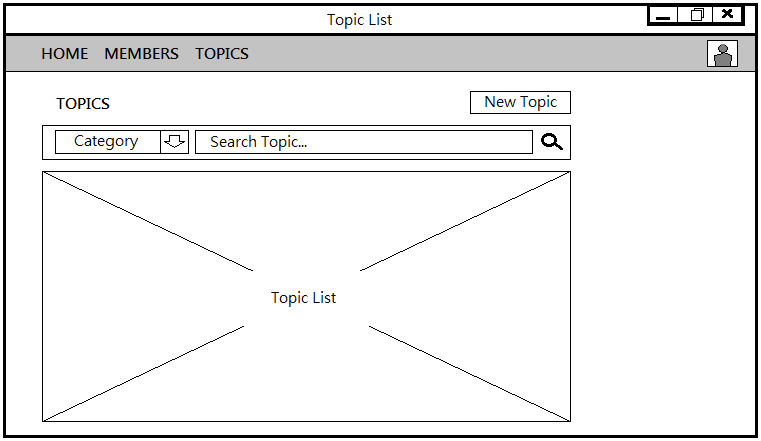
\includegraphics[width=.7\textwidth]{img/prototype/TopicList.png}
\caption{Prototype -- 文章列表頁面(含搜尋功能)}
\label{pic:pro:articleList}
\end{figure}

%% ####################### %%
\subsubsection{關係建立模組}

本系統中基於完成使用者之特定隱私權設計之理念,將在系統中提供建立好友關系的功能,也就是本模組的核心。本模組必須要能傳遞使用者的交友邀請、記錄使用者對於要求的回應與記錄使用者與其他用戶之關係。除了雙向之好友功能,本系統亦提供建立單項之關注其他使用者之功能。兩者的差異在於,好友是需要雙方合意,而可以使雙方看到對方之所有資訊;另一方面,關注關係不需要被關注者之同意,而系統僅於被關注者有發表新文章時會寄發通知信予關注者。本模組著重的重點在於資料抽象化之設計,更多細節請參考小節~\ref{sssec:following} 。

%% ####################### %%
\subsubsection{討論區模組}
討論區模組需包含以下三點功能:新增文章、瀏覽文章、標示文章類別。在新增文章時使用者將被要求選擇文章類別,以供其他使用者快速過濾想閱讀之訊息。由於系統沒有自動根據文章內容判斷其真實內容之能力,目前仍需仰賴使用者自動自發之行為來維持正確性,未來若能發展出足以將此行為自動化之方法則可降低系統在本問題之人力需求。此模組需同時提供標示文章類別與讓使用者方便瀏覽之功能,以達訊息交流之初衷。本模組將由前端網頁系統負責,只有將文章記錄至資料庫的行為需要後端資料系統輔助。

\begin{figure}[H]
\centering
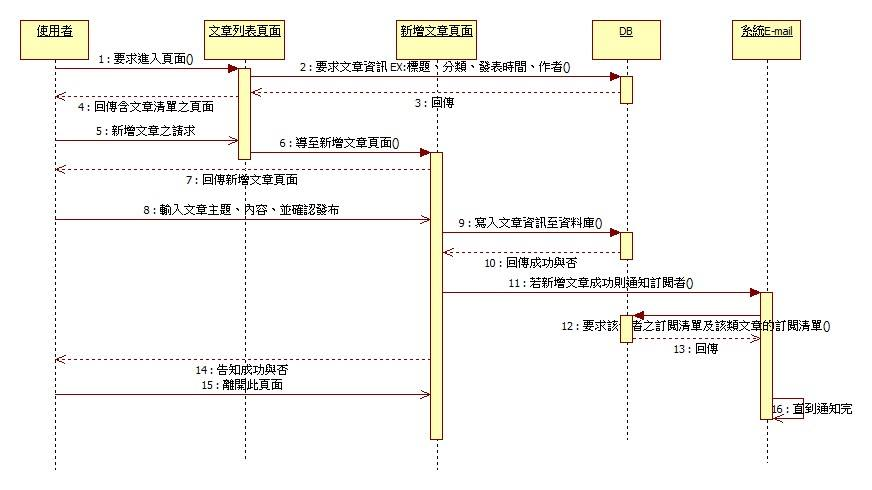
\includegraphics[width=1.05\textwidth]{img/useseq/stage2/seqNewArticle.jpg}
\caption{Sequence Diagram -- 新增文章}
\label{pic:seq:newArticle}
\end{figure}

\begin{figure}[H]
\centering
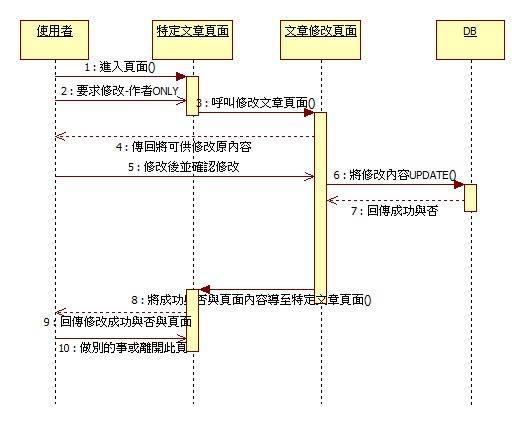
\includegraphics[width=.8\textwidth]{img/useseq/stage2/seqEditArticle.jpg}
\caption{Sequence Diagram -- 修改文章}
\label{pic:seq:editArticle}
\end{figure}

\begin{figure}[H]
\centering
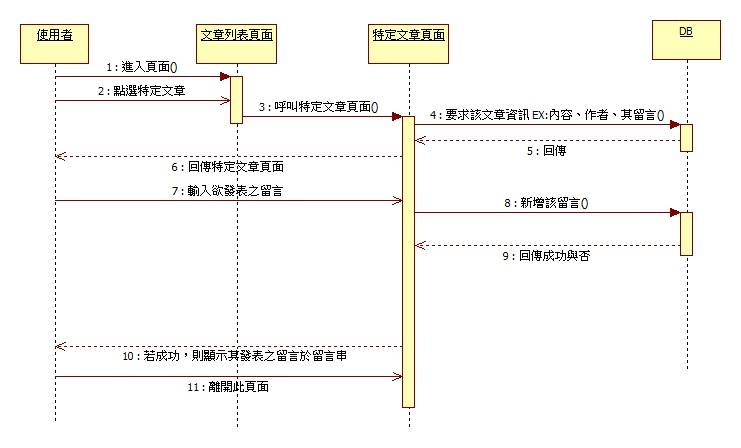
\includegraphics[width=1.05\textwidth]{img/useseq/stage2/seqNewComment.jpg}
\caption{Sequence Diagram -- 新增留言}
\label{pic:seq:newComment}
\end{figure}

%% ####################### %%
\subsubsection{訂閱模組}
\label{sssec:subscription}
訂閱模組中包含訂閱文章及訂閱文章類別等功能。訂閱之行為一致為當訂閱之目標有了內容之新增與改變時,將由後端信件系統發信至訂閱人所登記之信箱提醒使用者。訂閱文章的訂閱隊項為單篇文章,訂閱方法可包括在該文章留言或是點選訂閱按鈕,資料的改變為該文章被新增了評論時提醒。訂閱文章類別則將在任何一篇文章被標示為該類別時提醒使用者。本模組需由前端網頁系統展現、後端資料系統記錄與後端郵件系統共同合作完成。訂閱文章及文章分類請參考圖~\ref{pic:seq:search} 。

\begin{figure}[H]
\centering
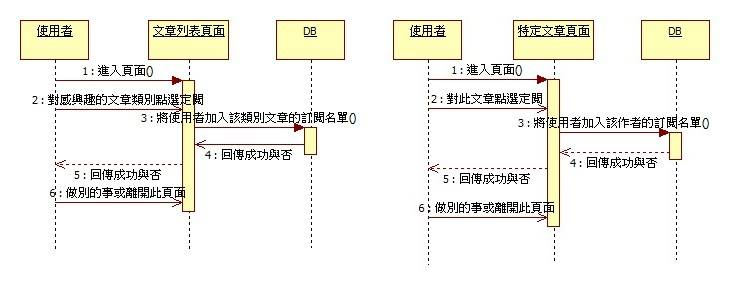
\includegraphics[width=\textwidth]{img/useseq/stage2/seqSearch.jpg}
\caption{Sequence Diagram -- 訂閱文章或文章分類}
\label{pic:seq:search}
\end{figure}



%% ####################### %%


%% ####################### %%
% first column
\begin{minipage}[t]{0.5\textwidth}
\subsubsection{API模組}

本系統基於 Grape,一個 REST-like API micro-framework,與 Ruby on Rails 整合,來提供系統 JSON API,並遵循 REST (Representational State Transfer) 的軟體架構風格實作,客戶端的應用通過 URI 來獲取資源的表徵,收取以 JSON 之資料格式來產生狀態的變化,對資源的操作包括獲取、創建、修改和刪除資源,這些操作對應於HTTP協議提供的 GET、POST、PUT 和 DELETE 方法。 以新增議題為例:當使用者需要新增議題時,透過客戶端程式來以 HTTP request Server,因為新增文章代表需創建新的資料,所以使用 POST 做為 HTTP request 的方法,並對其設定的URI(http://alumnibook.com/api/topics/)做 request,這樣 Server 就會判斷其 HTTP requset 參數來做相對應的回覆,若所夾帶參數通過檢驗即可建立新的議題,並回覆新增之議題的資料,若所夾帶參數未能通過檢驗,例如必須欄位未提供或是其資料格式錯誤,則會回傳錯誤訊息,API 所回傳的資料格式皆以 JSON 作為主要資料格式。API 最主要可以提供其他網站服務或是行動裝置端的程式使用,例如說圖~\ref{pic:seq:appi} 呈現了以手機程式為客戶端時,該服務與本系統之 API 之間可能的互動模式。
\end{minipage}
%second column
\begin{minipage}[t]{0.5\textwidth}
\begin{figure}[H]
\centering
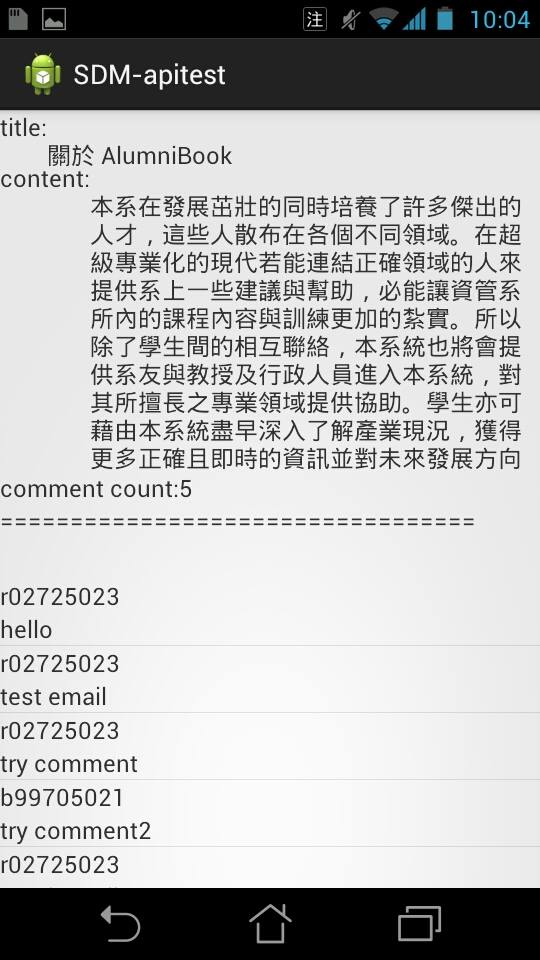
\includegraphics[width=0.65\textwidth]{img/prototype/android.jpg}
\caption{Android Screenshot -- 行動程式}
\label{pic:app}
\end{figure}
\end{minipage}

\subsubsection{行動程式}
行動裝置端的程式極其輕便,僅帶來快速的文章流覽功能。手機程式的執行畫面雛形如圖~\ref{pic:app} 所示。在手機端程式啟動後,程式會向API要求資料。在接收到伺服器端所提供的JSON陣列後,手機端會做一連串的處理動作。從該JSON陣列中一項一項抽取出來的資料在成功解構後會暫時以方便取用的格式放在本機端以供未來使用,並且先將使用者列表簡單的呈現給使用者。使用者選擇有興趣的文章時則可從本機端的資料中取得該篇文章的內文、作者以及評論。手機端程式與網站 API 之間的互動細節請參考圖~\ref{pic:seq:appi}。

\begin{figure}[H]
\centering
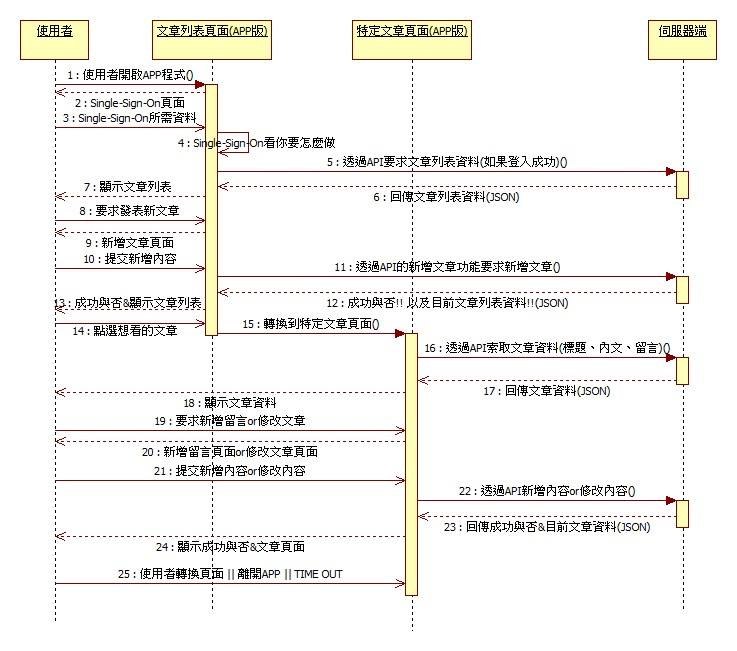
\includegraphics[width=\textwidth]{img/useseq/appi.jpg}
\caption{Sequence Diagram -- API and Android App}
\label{pic:seq:appi}
\end{figure}


